\documentclass{article}
\usepackage[T1]{fontenc}
\usepackage[utf8]{inputenc}
\usepackage[spanish]{babel}
\usepackage[pdftex]{graphicx}
\usepackage{geometry}
\usepackage{caratula}

\begin{document}

\newgeometry{left=2cm,right=2cm}

\titulo{Trabajo Práctico 1A: \emph{Wiretapping}}
%\subtitulo{Subtítulo del tp}

%\fecha{\today}

\materia{Teoría de las Comunicaciones}
%\grupo{Grupo 42}

\integrante{Antonio, Pablo}{290/08}{pabloa@gmail.com}
\integrante{Ferrari, Gastón}{775/07}{gastonferrari5@hotmail.com}

\maketitle

\newgeometry{left=5cm,right=5cm}

\tableofcontents

\newpage

\section{Introducción}
El presente informe corresponde al Trabajo Práctico 1A, titulado
"\emph{Wiretapping}", de la materia Teoría de las Comunicaciones. El objetivo
de este trabajo es desarrollar una herramienta sencilla de diagnóstico de red
y realizar un análisis a partir de la información que esta nos provee en
distintos segmentos de red.

\subsection{ARP}
El trabajo, en particular, se enfoca en el monitoreo de las interacciones
entre distintos \emph{hosts} mediante el protocolo ARP (\emph{Address
Resolution Protocol}). El objetivo de ARP es permitirle, a los \emph{hosts} de
una red, armar una tabla de asociaciones entre direcciones IP y direcciones de
nivel de enlace. Esta tabla de de asociaciones, presente en cada \emph{host},
se conoce como tabla ARP o \emph{cache} ARP.

Cuando un \emph{host} quiere enviar un datagrama IP a otro \emph{host} o
\emph{router} en la misma red, realiza lo siguiente:

\begin{enumerate}
    \item Verifica si en su tabla ARP existe una asociación para la dirección
        IP destino del datagrama.
    \item Si la hay, envía el datagrama a la dirección de nivel de enlace
        respectiva.
    \item Si no la hay, utiliza ARP para completar su tabla con la asociación
        necesaria, para así luego enviar el datagrama a la dirección de nivel
        de enlace respectiva.
\end{enumerate}

El mecanismo utilizado en este último caso consiste en enviar una consulta ARP
vía \emph{broadcast} a la red. La consulta (\emph{request}) de ARP contiene la
dirección IP de la que se desea conocer su dirección de nivel de enlace
asociada. Cada \emph{host} en la red, una vez que recibe esta consulta, se
ocupa de chequear si la IP por la que se consulta es la propia. En caso de que
así sea, el \emph{host} envía una respuesta (\emph{reply}) de ARP, que
contiene su dirección de nivel de enlace, al \emph{host} que hizo
originalmente la consulta para que este pueda, entonces, completar su tabla
ARP con la nueva asociaciación.

\subsection{Herramientas desarrolladas}
Para poder realizar los análisis, desarrollamos pequeñas herramientas que nos
sirvieron para monitorear la red y generar gráficos sobre el comportamiento de
esta.

Para el monitoreo de la red, escribimos un breve \emph{script} en Python que,
valiéndose de la biblioteca Scapy, nos permite generar archivos de texto con
entradas que describen las interacciones ARP entre los distintos \emph{hosts}
de la red.

Escribimos, también, dos \emph{scripts} más, que procesan los archivos de texto
antes nombrados y nos dan información relevante para nuestro posterior
análisis. El primer \emph{script} da como salida valores o medidas
relacionadas al análisis de las distintas fuentes de información que
definimos; por ejemplo, la entropía de cada fuente. El segundo \emph{script}
se ocupa de generar gráficos: De barras, y un grafo que relaciona \emph{hosts}
en la red que interactúan mediante el protocolo ARP.


\section{Análisis de las redes}
Para realizar el análisis de la red, desde un punto de vista de la Teoría de
la Información, elegimos tres fuentes de información diferentes:

\begin{itemize}
    \item Fuente cuyos símbolos son IPs que realizan una consulta
        (\emph{request}) vía el protocolo ARP.
    \item Fuente cuyos símbolos son IPs que responden una consulta
        (\emph{reply}) vía el protocolo ARP.
    \item Fuente cuyos símbolos son IPs por las que se realiza una consulta
        (\emph{request}) vía el protocolo ARP.
    \item Fuente cuyos símbolos son IPs que a las que le responden una
        consulta (\emph{reply}) vía el protocolo ARP.
\end{itemize}

Los datos fueron tomados de redes hogareñas.

\subsection{Red 1}
\subsubsection{Símbolos: IPs que realizan una consulta ARP}
La siguiente tabla muestra, para cada símbolo, su cantidad de apariciones y
sus medidas de probabilidad e información asociadas.

\vskip10pt

\begin{tabular}{|l|l|l|l|l|}
  \hline
  Símbolo & Apariciones & Probabilidad & Información \\
  \hline
  192.168.0.105 & 99 & $0.0947368421053$ & $3.39993060689$ \\
  \hline
  192.168.0.104 & 28 & $0.0267942583732$ & $5.22193230491$ \\
  \hline
  192.168.0.1 & 415 & $0.397129186603$  & $1.33231970073$ \\
  \hline
  192.168.0.101 & 448 & $0.428708133971$ & $1.22193230491$ \\
  \hline
  192.168.0.100 & 1 & $0.000956937799043$ & $10.029287227$ \\
  \hline
  192.168.0.103 & 11 & $0.0105263157895$ & $6.56985560833$ \\
  \hline
  192.168.0.102 & 26 & $0.0248803827751$ & $5.32884750883$ \\
  \hline
  0.0.0.0 & 17 & $0.0162679425837$ & $5.94182438572$ \\
  \hline
\end{tabular}

\vskip10pt

La entropía de la fuente es:

$$H(S) = 1.82297065237$$

En la figura \ref{fig:red1requesters:infoentro}, puede observarse gráficamente
los valores de información de cada símbolo en relación con la entropía de la
red.

\begin{figure}[h!]
    \centering                                                       
    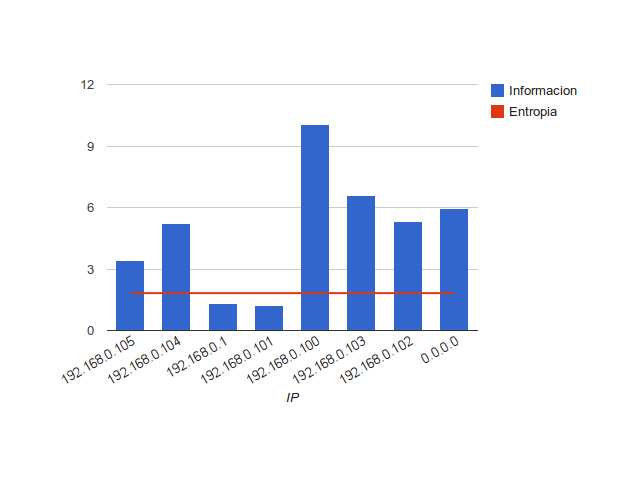
\includegraphics[width=300pt]{consultas1.png}
    \caption{Información de cada símbolo, en relación con la
        entropía de la red}
    \label{fig:red1requesters:infoentro}
\end{figure}

La figura \ref{fig:red1requesters:count} muestra la cantidad de apariciones de
cada símbolo.

\begin{figure}[h!]
    \centering                                                       
    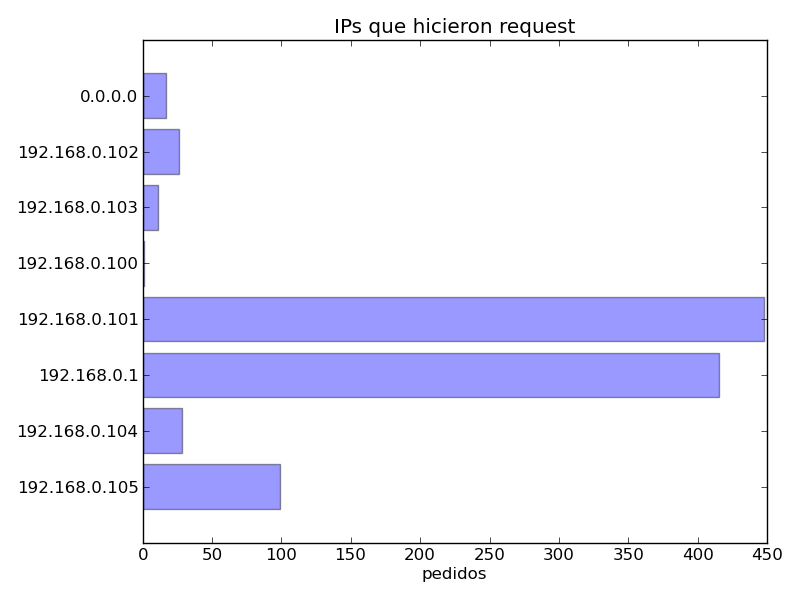
\includegraphics[width=300pt]{red1requesters.png}
    \caption{Apariciones de los símbolos}
    \label{fig:red1requesters:count}
\end{figure}

La figura \ref{fig:red1requesters:graph} permite observar qué IPs realizaron
consultas sobre qué otras IPs de la red. El tamaño de cada nodo se corresponde
con la cantidad de pedidos que realizó cada IP.

\begin{figure}[h!]
    \centering
    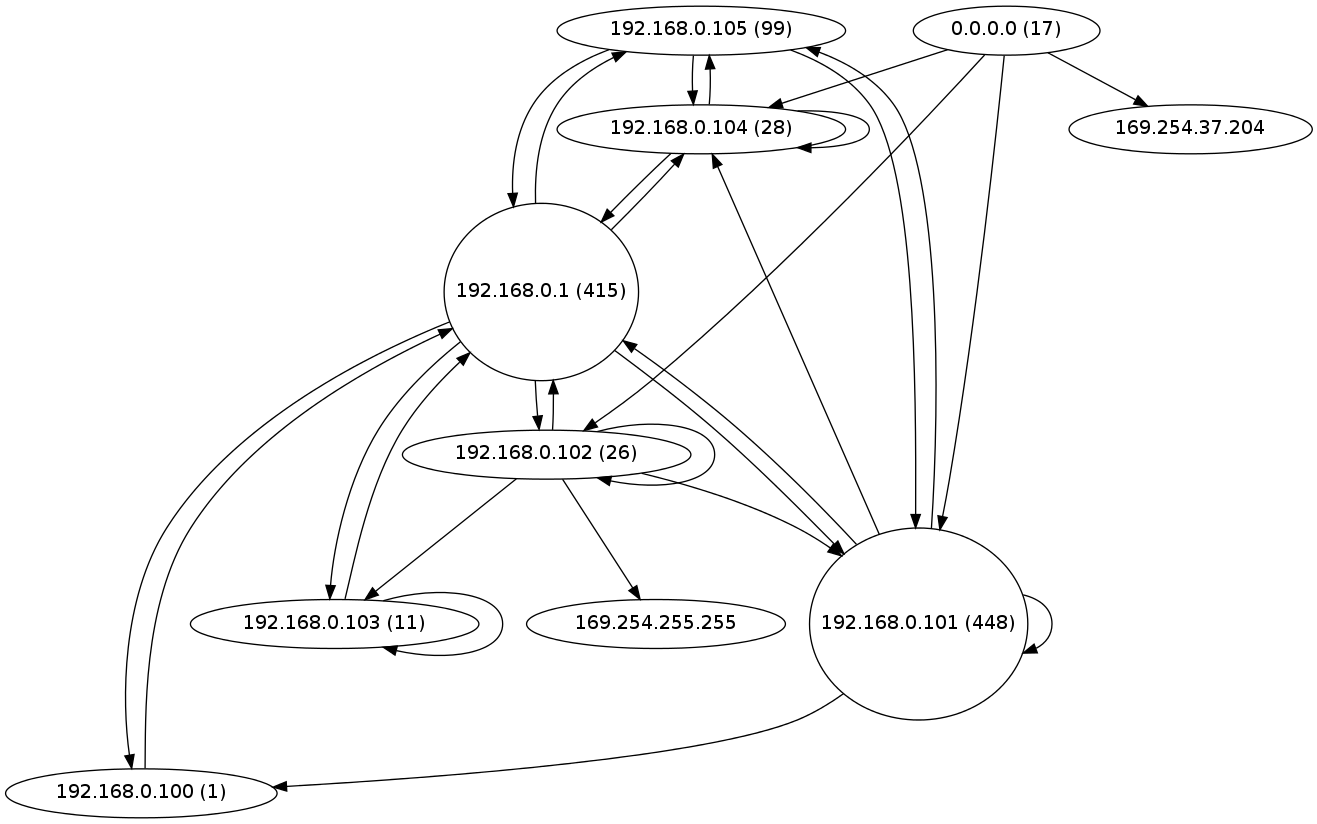
\includegraphics[width=350pt]{red1requestersgraph.png}
    \caption{Grafo en el que hay un eje desde una IP A a una IP B si la IP A
        realizó una consulta por la IP B}
    \label{fig:red1requesters:graph}
\end{figure}

En estos gráficos se observa claramente que los \emph{hosts} 192.168.0.1 y
192.168.0.101 se destacan, tanto por la cantidad de pedidos que realizan como
por la cantidad de \emph{hosts} con los que interactúan.

La IP 192.168.0.1 corresponde al \emph{router} presente en la red. Es lógico,
entonces, que la cantidad de pedidos que este realiza sea tan alta, dado que
es el encargado de distribuir todo el tráfico de la red a los \emph{hosts}
correspondientes. Por esto, su tabla de direcciones MAC tiene que estar
correctamente actualizada el mayor tiempo posible.

Por otro lado, la IP 192.168.0.101 corresponde a un \emph{host} que sirve de
servidor de archivos para el resto de la red. De allí que interactue con
tantos otros \emph{hosts} y que envíe tantos pedidos ARP.

\subsubsection{Símbolos: IPs que responden una consulta ARP}
La siguiente tabla muestra, para cada símbolo, su cantidad de apariciones y
sus medidas de probabilidad e información asociadas.

\vskip10pt

\begin{tabular}{|l|l|l|l|l|}
  \hline
  Símbolo & Apariciones & Probabilidad & Información \\
  \hline
  192.168.0.105 & 506 & $0.85472972973$ & $0.226459790935$ \\
  \hline
  192.168.0.101 & 24 & $0.0405405405405$ & $4.62449086491$ \\
  \hline
  192.168.0.1 & 62 & $0.10472972973$ & $3.25525705524$ \\
  \hline
\end{tabular}\\

\vskip10pt

La entropía de la fuente es:

$$H(S) = 0.721963466885$$

En la figura \ref{fig:red1repliers:infoentro}, puede observarse gráficamente
los valores de información de cada símbolo en relación con la entropía de la
red.

\begin{figure}[h!]
    \centering                                                       
    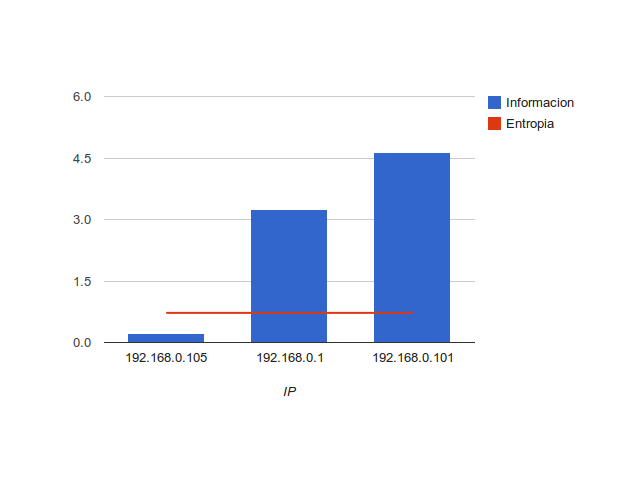
\includegraphics[width=300pt]{respuestas1.png}
    \caption{Información de cada símbolo, en relación con la
        entropía de la red}
    \label{fig:red1repliers:infoentro}
\end{figure}

La figura \ref{fig:red1repliers:count} muestra la cantidad de apariciones de
cada símbolo.

\begin{figure}[h!]
    \centering
    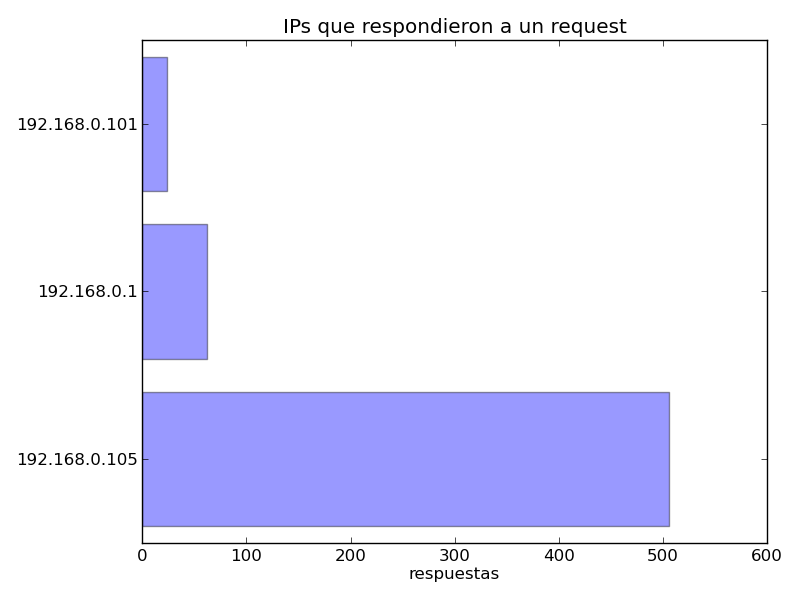
\includegraphics[width=300pt]{red1repliers.png}
    \caption{Apariciones de los símbolos}
    \label{fig:red1repliers:count}
\end{figure}

En este caso, la IP 192.168.0.105 fue la que más veces contestó los pedidos
sobre su dirección MAC; de ahí su probabilidad tan alta. Como se puede
observar, la información aportada por este símbolo es considerablemente más
baja que la aportada por los demás que poseen menor probabilidad. Incluso, la
información que representa es más baja que la entropía de la fuente.

\subsubsection{Símbolos: IPs por las que se realiza una consulta ARP}
La siguiente tabla muestra, para cada símbolo, su cantidad de apariciones y
sus medidas de probabilidad e información asociadas.

\vskip10pt

\begin{tabular}{|l|l|l|l|l|}
  \hline
  Símbolo & Consultas & Probabilidad & Información \\
  \hline
  169.254.37.204 & 3 & $0.00287081339713$ & $8.44432472625$\\
  \hline
  192.168.0.105 & 506 & $0.484210526316$ & $1.04629365227$\\
  \hline
  192.168.0.104 & 52 & $0.0497607655502$ & $4.32884750883$\\
  \hline
  169.254.255.255 & 10 & $0.00956937799043$ & $6.70735913208$\\
  \hline
  192.168.0.1 & 88 & $0.0842105263158$ & $3.56985560833$\\
  \hline
  192.168.0.101 & 30 & $0.0287081339713$ & $5.12239663136$\\
  \hline
  192.168.0.100 & 316 & $0.302392344498$ & $1.72550647879$\\
  \hline
  192.168.0.103 & 18 & $0.0172248803828$ & $5.85936222553$\\
  \hline
  192.168.0.102 & 22 & $0.0210526315789$ & $5.56985560833$\\
  \hline
\end{tabular}

\vskip10pt

La entropía de la fuente es:

$$H(S) = 1.99810125093$$

En la figura \ref{fig:red1requested:infoentro}, puede observarse gráficamente
los valores de información de cada símbolo en relación con la entropía de la
red.

\begin{figure}[h!]
    \centering                                                       
    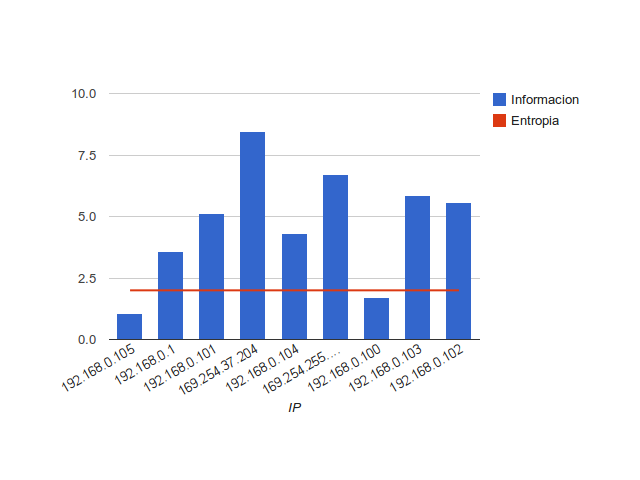
\includegraphics[width=300pt]{consultadas1.png}
    \caption{Información de cada símbolo, en relación con la
        entropía de la red}
    \label{fig:red1requested:infoentro}
\end{figure}

La figura \ref{fig:red1requested:count} muestra la cantidad de apariciones de
cada símbolo.

\begin{figure}[h!]
    \centering
    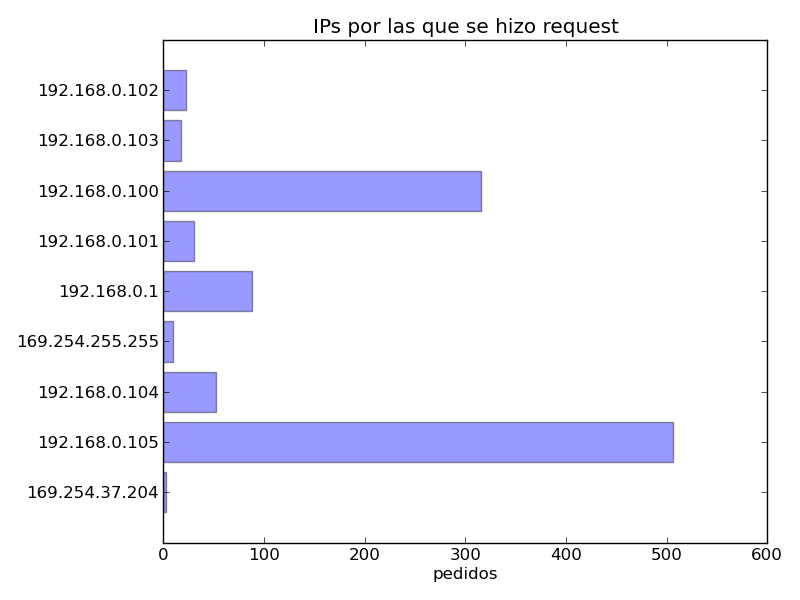
\includegraphics[width=300pt]{red1requested.png}
    \caption{Apariciones de los símbolos}
    \label{fig:red1requested:count}
\end{figure}

En este caso, la IP más consultada en la red fue la 192.168.0.105. Esto tiene
sentido, dado que, como vimos, es la que más respuestas dio. Al igual que en
el punto anterior, por consecuencia de su alta probabilidad de aparecer en la
fuente, su información no supera a la entropía que ofrece la red. Estimamos
que simplemente se trata de un \emph{host} muy activo en el uso de los
servicios de la red.

\subsubsection{Símbolos: IPs a las que le respondieron una consulta ARP}
La siguiente tabla muestra, para cada símbolo, su cantidad de apariciones y
sus medidas de probabilidad e información asociadas.

\vskip10pt

\begin{tabular}{|l|l|l|l|l|}
  \hline
  Símbolo & Consultas & Probabilidad & Información \\
  \hline
  192.168.0.105 & 86.0 & 0.14527027027 & 2.78318861093\\
  \hline
  192.168.0.104 & 21.0 & 0.035472972973 & 4.81713594285\\
  \hline
  192.168.0.1 & 84.0 & 0.141891891892 & 2.81713594285\\
  \hline
  192.168.0.101 & 401.0 & 0.677364864865 & 0.561994939174\\
  \hline

\end{tabular}

\vskip10pt

La entropía de la fuente es:

$$H(S) = 1.35559706951$$

En la figura \ref{fig:red1replied:infoentro}, puede observarse gráficamente
los valores de información de cada símbolo en relación con la entropía de la
red.

\begin{figure}[h!]
    \centering                                                       
    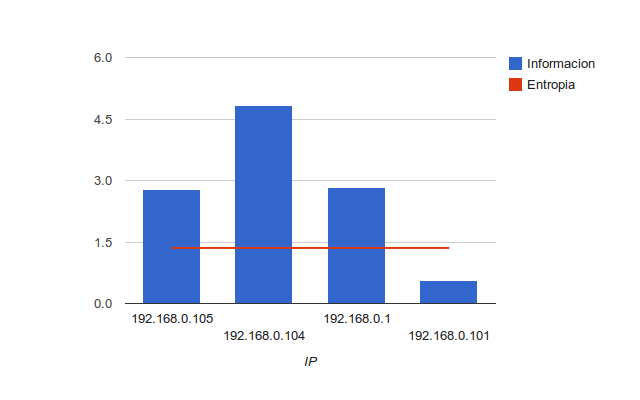
\includegraphics[width=300pt]{respondidas1.png}
    \caption{Información de cada símbolo, en relación con la
        entropía de la red}
    \label{fig:red1replied:infoentro}
\end{figure}

La figura \ref{fig:red1replied:count} muestra la cantidad de apariciones de
cada símbolo.

\begin{figure}[h!]
    \centering
    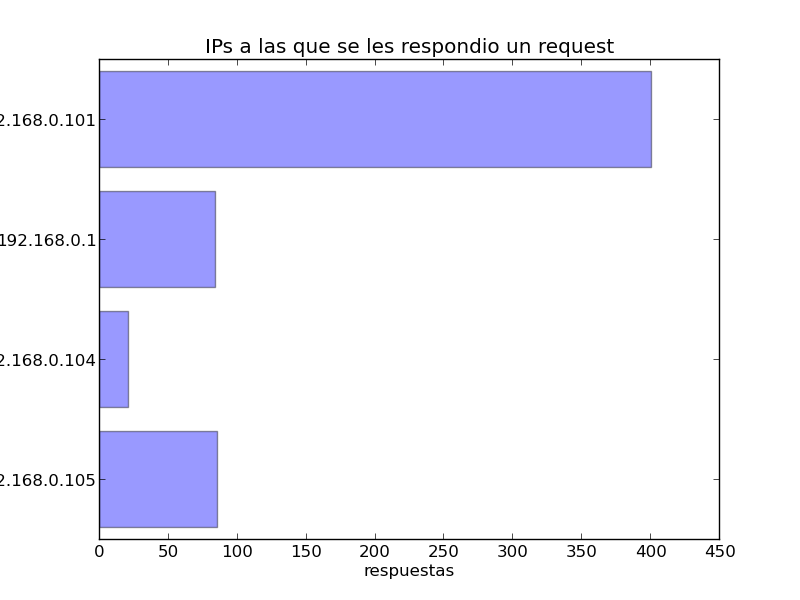
\includegraphics[width=300pt]{red1replied.png}
    \caption{Apariciones de los símbolos}
    \label{fig:red1replied:count}
\end{figure}

Aquí podemos observar que, si bien tanto la IP 192.168.0.1 (el \emph{router})
como la IP 192.168.0.101 (servidor de archivos) realizaron ambas más de 400
pedidos ARP, existe una gran disparidad en la cantidad de respuestas que estas
recibieron. Esto puede deberse a muchas razones. Por ejemplo, a cuestiones
físicas de la red que ocasionan pérdidas de paquetes, o a que algunos
\emph{hosts} hacen consultas por su propia IP para asegurarse que no está
duplicada en la red.

En este caso particular, al analizar los datos, observamos que el
\emph{router} realiza una gran cantidad de consultas por la IP 192.168.0.100 y
el \emph{host} asociado a esta IP nunca responde. Esto puede deberse a
problemas físicos en la red o a una falla o bloqueo intencional en el
\emph{host} en cuestión.


%%%%%%%%%%%%%%%%%%%%%%%%%%%%%%%%%%%%%%%%%%%%%%%%%%%%%%%%%%%%%%%%%%%%%%%
%*********************************************************************%
%*********************************************************************%
%******************************RED 2**********************************%
%*********************************************************************%
%*********************************************************************%
%%%%%%%%%%%%%%%%%%%%%%%%%%%%%%%%%%%%%%%%%%%%%%%%%%%%%%%%%%%%%%%%%%%%%%%

\subsection{Red 2}
\subsubsection{Símbolos: IPs que realizan una consulta ARP}
La siguiente tabla muestra, para cada símbolo, su cantidad de apariciones y
sus medidas de probabilidad e información asociadas.

\vskip10pt

\begin{tabular}{|l|l|l|l|l|}
  \hline
  Símbolo & Apariciones & Probabilidad & Información \\
  \hline
  192.168.0.105 & 57.0 & 0.0578093306288 & 4.11255382221\\
\hline
192.168.0.1 & 770.0 & 0.78093306288 & 0.356729200796\\
\hline
192.168.0.101 & 59.0 & 0.0598377281947 & 4.06280078702\\
\hline
192.168.0.100 & 3.0 & 0.00304259634888 & 8.36048133566\\
\hline
192.168.0.102 & 92.0 & 0.0933062880325 & 3.42188188032\\
\hline
0.0.0.0 & 5.0 & 0.00507099391481 & 7.62351574149\\
\hline

\end{tabular}

\vskip10pt

La entropía de la fuente es:

$$H(S) = 1.1428138485$$

En la figura \ref{fig:red2requesters:infoentro}, puede observarse gráficamente
los valores de información de cada símbolo en relación con la entropía de la
red.

\begin{figure}[h!]
    \centering                                                       
    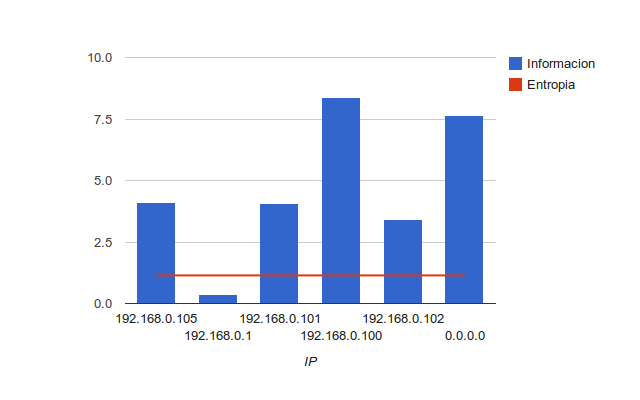
\includegraphics[width=300pt]{red2/consultas2.png}
    \caption{Información de cada símbolo, en relación con la
        entropía de la red}
    \label{fig:red2requesters:infoentro}
\end{figure}

La figura \ref{fig:red2requesters:count} muestra la cantidad de apariciones de
cada símbolo. Nuevamente podemos observar que la IP 192.168.0.1 (router) es la que más pedidos realiza.

\begin{figure}[h!]
    \centering                                                       
    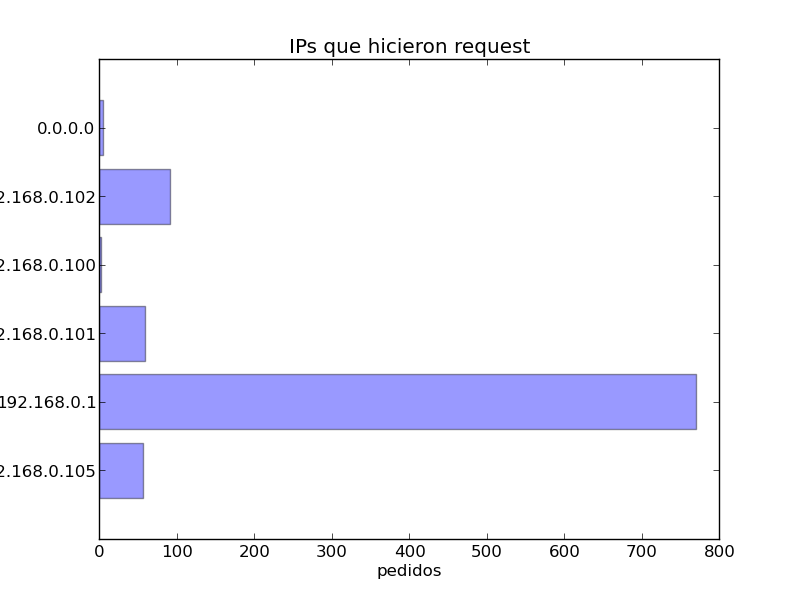
\includegraphics[width=300pt]{red2/red2requesters.png}
    \caption{Apariciones de los símbolos}
    \label{fig:red2requesters:count}
\end{figure}

La figura \ref{fig:red2requesters:graph} permite observar qué IPs realizaron
consultas sobre qué otras IPs de la red. El tamaño de cada nodo se corresponde
con la cantidad de pedidos que realizó cada IP.

\begin{figure}[h!]
    \centering
    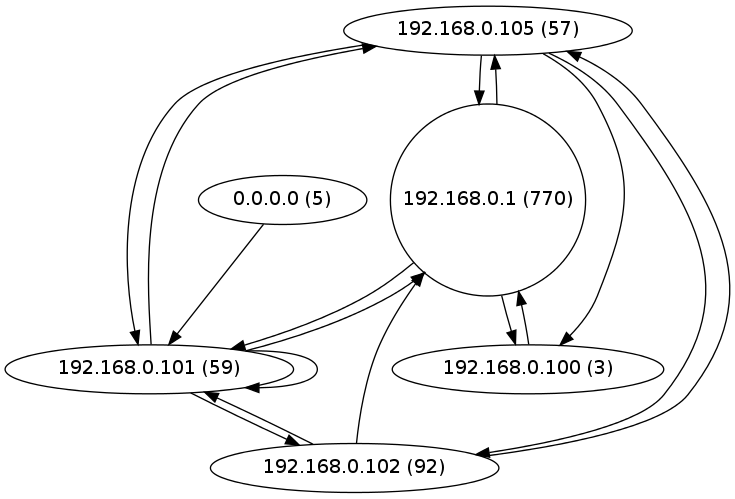
\includegraphics[width=350pt]{red2/red2requestersgraph.png}
    \caption{Grafo en el que hay un eje desde una IP A a una IP B si la IP A
        realizó una consulta por la IP B}
    \label{fig:red2requesters:graph}
\end{figure}


\newpage

\subsubsection{Símbolos: IPs que responden una consulta ARP}
La siguiente tabla muestra, para cada símbolo, su cantidad de apariciones y
sus medidas de probabilidad e información asociadas.

\vskip10pt

\begin{tabular}{|l|l|l|l|l|}
  \hline
  Símbolo & Apariciones & Probabilidad & Información \\
  \hline
  192.168.0.105 & 134.0 & 0.732240437158 & 0.449610647826\\
\hline
192.168.0.1 & 36.0 & 0.196721311475 & 2.34577483684\\
\hline
192.168.0.100 & 3.0 & 0.016393442623 & 5.93073733756\\
\hline
192.168.0.102 & 10.0 & 0.0546448087432 & 4.1937717434\\
\hline
\end{tabular}\\

\vskip10pt

La entropía de la fuente es:
$$H(S) = 1.11708005673$$

En la figura \ref{fig:red2repliers:infoentro}, puede observarse gráficamente
los valores de información de cada símbolo en relación con la entropía de la
red.

\begin{figure}[h!]
    \centering                                                       
    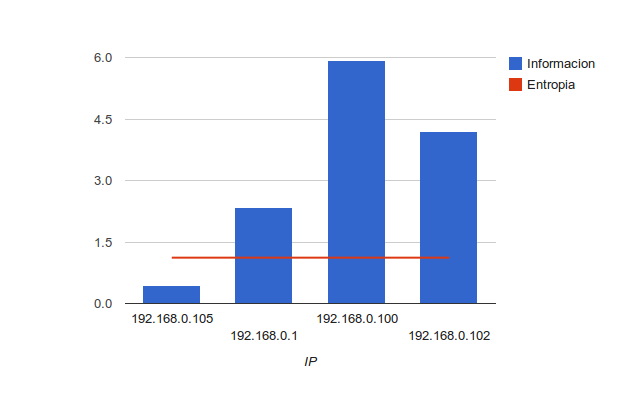
\includegraphics[width=300pt]{red2/respuestas2.png}
    \caption{Información de cada símbolo, en relación con la
        entropía de la red}
    \label{fig:red2repliers:infoentro}
\end{figure}

La figura \ref{fig:red2repliers:count} muestra la cantidad de apariciones de
cada símbolo.

\begin{figure}[h!]
    \centering
    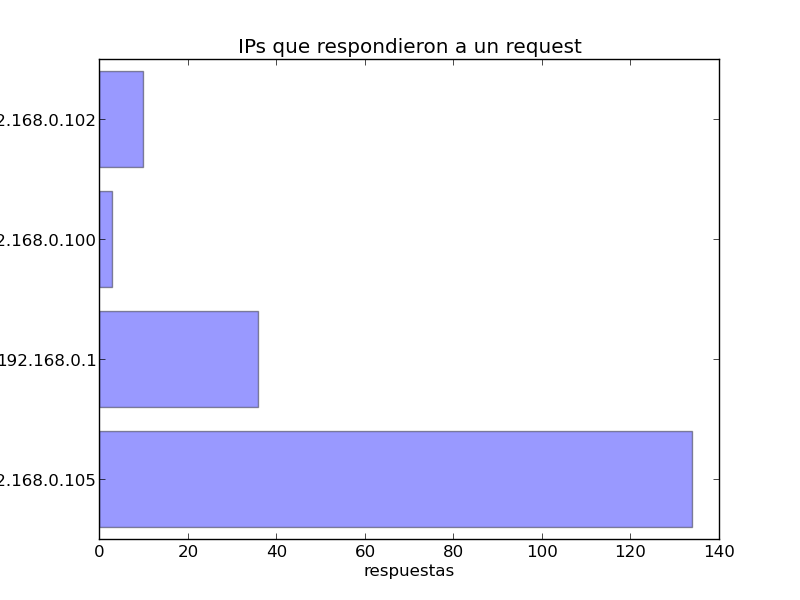
\includegraphics[width=300pt]{red2/red2repliers.png}
    \caption{Apariciones de los símbolos}
    \label{fig:red2repliers:count}
\end{figure}


\newpage

\subsubsection{Símbolos: IPs por las que se realiza una consulta ARP}
La siguiente tabla muestra, para cada símbolo, su cantidad de apariciones y
sus medidas de probabilidad e información asociadas.

\vskip10pt

\begin{tabular}{|l|l|l|l|l|}
  \hline
  Símbolo & Consultas & Probabilidad & Información \\
  \hline
  192.168.0.105 & 134.0 & 0.135902636917 & 2.87935464592\\
\hline
192.168.0.1 & 51.0 & 0.051724137931 & 4.27301849441\\
\hline
192.168.0.101 & 86.0 & 0.0872210953347 & 3.51917908168\\
\hline
192.168.0.100 & 704.0 & 0.713995943205 & 0.486012217741\\
\hline
192.168.0.102 & 11.0 & 0.0111561866126 & 6.48601221774\\
\hline
\end{tabular}

\vskip10pt

La entropía de la fuente es:

$$H(S) = 1.33864665566$$

En la figura \ref{fig:red2requested:infoentro}, puede observarse gráficamente
los valores de información de cada símbolo en relación con la entropía de la
red.

\begin{figure}[h!]
    \centering                                                       
    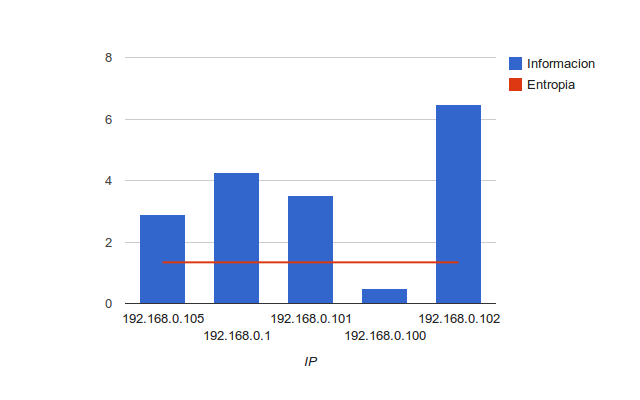
\includegraphics[width=300pt]{red2/consultadas2.png}
    \caption{Información de cada símbolo, en relación con la
        entropía de la red}
    \label{fig:red2requested:infoentro}
\end{figure}

La figura \ref{fig:red2requested:count} muestra la cantidad de apariciones de
cada símbolo.

\begin{figure}[h!]
    \centering
    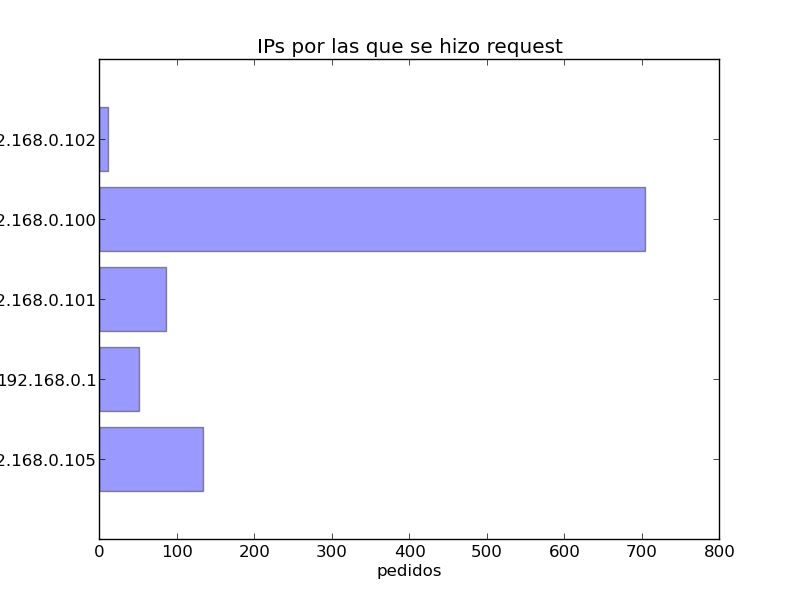
\includegraphics[width=300pt]{red2/red2requested.png}
    \caption{Apariciones de los símbolos}
    \label{fig:red2requested:count}
\end{figure}

\newpage

\subsubsection{Símbolos: IPs a las que le respondieron una consulta ARP}
La siguiente tabla muestra, para cada símbolo, su cantidad de apariciones y
sus medidas de probabilidad e información asociadas.

\vskip10pt

\begin{tabular}{|l|l|l|l|l|}
  \hline
  Símbolo & Consultas & Probabilidad & Información \\
  \hline
  192.168.0.105 & 49.0 & 0.267759562842 & 1.90098999417\\
\hline
192.168.0.1 & 67.0 & 0.366120218579 & 1.44961064783\\
\hline
192.168.0.101 & 50.0 & 0.273224043716 & 1.87184364851\\
\hline
192.168.0.102 & 17.0 & 0.0928961748634 & 3.42823699703\\
\hline
\end{tabular}

\vskip10pt

La entropía de la fuente es:

$$H(S) = 1.86964281144$$

En la figura \ref{fig:red2replied:infoentro}, puede observarse gráficamente
los valores de información de cada símbolo en relación con la entropía de la
red.

\begin{figure}[h!]
    \centering                                                       
    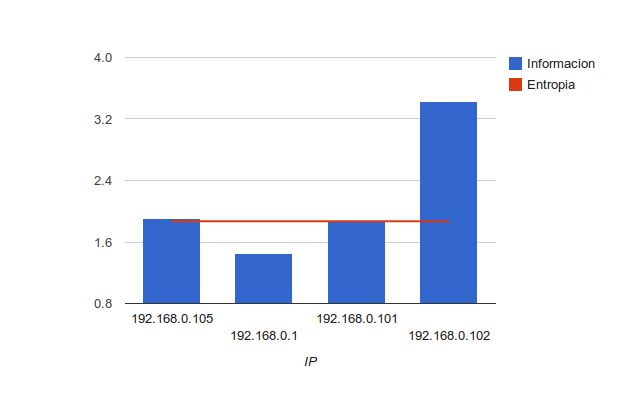
\includegraphics[width=300pt]{red2/respondidas2.png}
    \caption{Información de cada símbolo, en relación con la
        entropía de la red}
    \label{fig:red2replied:infoentro}
\end{figure}

La figura \ref{fig:red2replied:count} muestra la cantidad de apariciones de
cada símbolo.

\begin{figure}[h!]
    \centering
    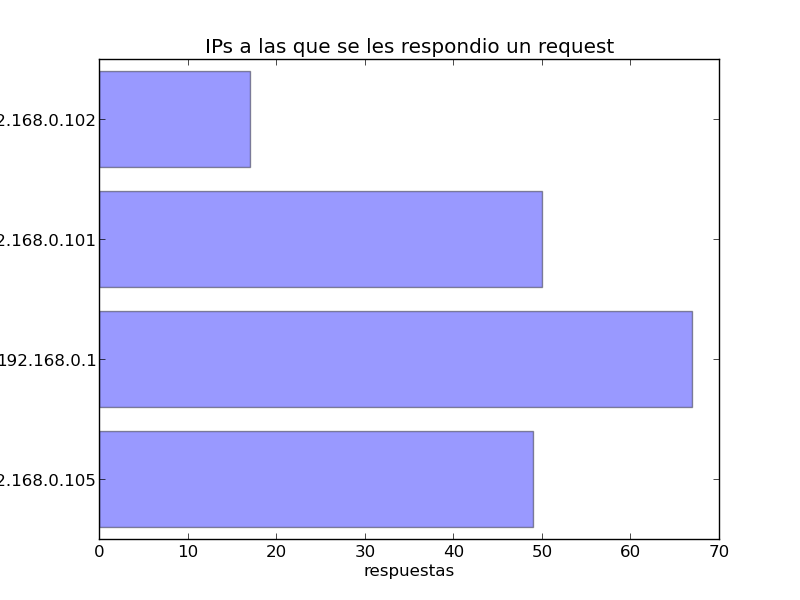
\includegraphics[width=300pt]{red2/red2replied.png}
    \caption{Apariciones de los símbolos}
    \label{fig:red2replied:count}
\end{figure}


%%%%%%%%%%%%%%%%%%%%%%%%%%%%%%%%%%%%%%%%%%%%%%%%%%%%%%%%%%%%%%%%%%%%%%%
%*********************************************************************%
%*********************************************************************%
%***************************CONCLUSION********************************%
%*********************************************************************%
%*********************************************************************%
%%%%%%%%%%%%%%%%%%%%%%%%%%%%%%%%%%%%%%%%%%%%%%%%%%%%%%%%%%%%%%%%%%%%%%%

\section{Conclusiones}
El trabajo nos permitió conocer el funcionamiento del protocolo ARP y observar
su uso en redes reales. Además de lo ya comentado anteriormente, de la
observación e investigación surgieron algunas conclusiones:

\begin{itemize}
    \item El protocolo ARP es muy importante, ya que resuelve el problema de
        traducción entre direcciones de nivel de red y direcciones de nivel de
        enlace. Su función es crítica en las redes de acceso múltiple y, si
        bien es usado comúnmente para traducir direcciones IP en direcciones
        ethernet, se ha implementado para la traducción entre diversos
        protocolos.
    \item El \emph{router} es siempre uno de los nodos más activos en la red
        y, a partir de la simple observación de los datos, es muy sencillo
        identificarlo. Esto tiene sentido, ya que la mayor parte del tráfico
        de la red pasa por él.
    \item Nos llamó la atención que la IP 0.0.0.0 apareciera como IP fuente de
        algunos pedidos. Investigando un poco, llegamos a la conclusión que
        esto sucede cuando un host recién se conecta a la red y se hace para
        verificar que no haya otro host con la misma IP.
    \item Al trabajar con el protocolo, notamos que este no es seguro, ya que
        permite que un \emph{host} se haga pasar por otro, respondiendo
        mensajes ARP que no estaban dirigidos a él. Esto se conoce como ARP
        \emph{spoofing}.
    \item Generalmente, los nodos distinguidos en la red aparecían, en las
        mediciones, con información menor a la entropía de la red. Esto tiene
        sentido, dado que la entropía puede interpretarse como la información
        media por símbolo emitida por la fuente. Cuando se esperaba que el
        símbolo ligado a un nodo apareciera mucho, la información que
        representaba su aparición era escasa. 
\end{itemize}


\section{Referencias}
\begin{itemize}
    \item Peterson, L. y Davie, B. (2007) Computer Networks: A Systems
        Approach: Morgan Kaufmann.
    \item Abramson, N. (1981) Teoría de la Información y Codificación:
        Paraninfo.
    \item Sitio web del proyecto Scapy: http://www.secdev.org/projects/scapy/
    \item Artículos de Wikipedia acerca de: Address Resolution Protocol, 
        Entropy (information theory).
\end{itemize}

\end{document}
